\chapter{Implementation}
\label{Implementation}

In this chapter we will outline the program structure, and we will
demonstrate the flexibility as well as the limitations of our
implementation. The program code developed in this thesis consists of
about $7000$ lines and more than $25$ different classes. We therefore
limits the description of the code, and focus on the key
building-blocks of the VMC algorithm. The full code is provided as an
appendix, in the hope that the comments therein, and
the description provided in this chapter, can help clearify the
different aspects of the VMC implementation.
\newline
%
\newline
Several computers may work for days solving even simple looking
physical problems. Therefore, a great deal of effort must be
put into the design and development of the numerical algorithms.
Three major concepts concerning the implementation of a
large program are

\begin{enumerate}
  \item{} Speed       - the computational time (CPU).
  \item{} Flexibility - the ability to handle many different special cases.
  \item{} Readability - how easy it is to understand the program (and
  make modifications).
\end{enumerate}

To acquire a fast running program the number of calculations must be
kept at a minimum. This often requires storing a lot of information so
that the same calculations are not performed multiple times. 
\newline
%
\newline
In order to obtain a flexible program, the program should consist of
many small building blocks that can easily be replaced by other similar
blocks. We want the blocks to work independently of each other. In
this way changing one block will not affect the others. But, at the
same time we want to keep the flow of data at a minimum.
\newline
%
\newline
The program structure should also
be easy to read. Often, modifications of existing programs need to be
done, either by the programmers themselves, or by other users. This
task can be very time consuming, especially if the program is
difficult to understand. The algorithms and data structure need to be
well documented, and the variables and building blocks should have
names that are logical.
\newline
%
\newline
When making a large program the three criteria cannot all be met to a
full extent, and compromises have to be made. The two most important
parts of our program are the Slater 
determinant part and the part including correlation
effects. Our first concern will be the program 
speed. Second, is the need for flexibility. We want to test different
one-particle orbitals in the Slater determinant as well as different
Jastrow-factors for the correlation. The unfortunate effect of
reducing the CPU time and increasing the flexibility is the
program becoming less transparent. 
\newline
%
\newline
Generating a good code for scientific purposes is a continuous
process, and the final program may differ considerably from the original
outline. Numerical tests of different algorithms gives insight along
the way, and the data structure is modified accordingly. 
Another problem is interconnected data; the data of one block often
depends on the changes done in a different block. Changing data in one
block can therefore have consequences in a completely different
part of the program. As a result, good routines to control the
data-flow should be established.





%%%%%%%%%%%%%%%%%%%%%%%%%%%%%%%%%%%%%%%%%%%%%%%%%%%%%%%%%%%%%%%%%%%%
%                                                                  %
%                      Structure of the QMC Program                %
%                                                                  %
%%%%%%%%%%%%%%%%%%%%%%%%%%%%%%%%%%%%%%%%%% %%%%%%%%%%%%%%%%%%%%%%%%%
\section{Structure of the QMC Program}
\label{StructureOfTheQMCProgram}

Our first concern is to recognize how we want the program to operate, and
to work out a program structure. We divide the program into blocks,
with each block performing a few specific tasks. Figure
\ref{program_structure} illustrates the principal building blocks of
our main program.

\begin{figure}[hbtp]
\begin{center}
  \input{Implementation/program.eepic}
  %\epsfig{file=Implementation/program.eps, height=8cm}
  \caption{Variational Monte-Carlo program structure}
  \label{program_structure}
\end{center}
\end{figure}

These blocks are again divided into smaller blocks as will be
outlined in this section. All input is handled by the \emph{Domain}
class. The user-specified input tells the program what to do. In our
program the input consists of several files that are associated with
different parts of the code. Here the trial wave-function is chosen
and variational parameters are set. The input specifies whether
we will optimize the variational parameters with respect to energy or
variance optimization. Several other variables are also chosen, such
as the acceptance ratio, number of thermalization steps, number of
cycles, whether we allow interchange of spin between
electrons, and the name of the output file\footnote{When we are
  running parallel computations by MPI, we generate several
  output-files.}.
\newline
%
\newline
In the Metropolis test the ratio

\begin{equation*}
  \frac{|\Psi(\mathbf{X}^{new})|^2}{|\Psi(\mathbf{X}^{old})|^2}.
\end{equation*}

is needed. When evaluating the local energy we also need the first and
second derivatives. These three factors constitutes the most
time-demanding part of the VMC algorithm. In this thesis the trial
wave-function we want to optimized have the general form

\begin{equation}
  \Psi_{\mathbf{\alpha}} = D_{\mathbf{\alpha}}^{\uparrow}
  D_{\mathbf{\alpha}}^{\downarrow} G_{\beta}.
\label{trialWaveFunctionForm}
\end{equation}

This allow us to treat the Slater determinant part and the part
concering the Jastrow-factor separately, which is seen because

\begin{equation}
  \frac{\Psi_{\mathbf{\alpha}}(\mathbf{X}^{new})}
       {\Psi_{\mathbf{\alpha}}(\mathbf{X}^{old})} =
  \frac{D_{\mathbf{\alpha}}^{\uparrow}(\mathbf{X}^{new})}
       {D_{\mathbf{\alpha}}^{\uparrow}(\mathbf{X}^{old})} +
  \frac{D_{\mathbf{\alpha}}^{\downarrow}(\mathbf{X}^{new})}
       {D_{\mathbf{\alpha}}^{\downarrow}(\mathbf{X}^{old})}
  \frac{G_{\beta}(\mathbf{X}^{new})} +
       {G_{\beta}(\mathbf{X}^{old})},    
\label{trialWaveFunctionRatio}
\end{equation}

and

\begin{equation}
  \frac{ \nabla \Psi_{\mathbf{\alpha}} }{ \Psi_{\mathbf{\alpha}} } 
  = \frac{ \nabla D_{\mathbf{\alpha}}^{\uparrow}   }
  { D_{\mathbf{\alpha}}^{\uparrow} }
  + \frac{ \nabla D_{\mathbf{\alpha}}^{\downarrow} }
  { D_{\mathbf{\alpha}}^{\downarrow} }
  + \frac{ \nabla G_{\beta}                        }
  { G_{\beta} },
\label{trialWaveFunctionGradient}
\end{equation}

and finally

\begin{equation}
  \frac{ \nabla^2 \Psi_{\mathbf{\alpha}} }{ \Psi_{\mathbf{\alpha}} } 
  = \frac{ \nabla^2 D_{\mathbf{\alpha}}^{\uparrow}   }
  { D_{\mathbf{\alpha}}^{\uparrow} }
  + \frac{ \nabla^2 D_{\mathbf{\alpha}}^{\downarrow} }
  { D_{\mathbf{\alpha}}^{\downarrow} }
  + \frac{ \nabla^2 G_{\beta}                        }
  { G_{\beta} }.
\label{trialWaveFunctionLaplacian}
\end{equation}


%%%%%%%%%%%%%%% Optimizing the Slater Determinant %%%%%%%%%%%%%%%%
\section{Optimizing the Slater Determinant}
\label{OptimizingTheSlaterDeterminant}

Determining a determinant of an $N \times N$ matrix by
standard Gaussian elimination is of the order of ${\cal O}(N^3)$
calculations. As there are $N\cdot d$ independent coordinates we need
to evaluate $N\cdot d$ Slater determinants for the gradient and
$N\cdot d$ for the Laplacian\footnote{In this thesis three-dimensional
  atoms will be considered. However, the program allows varying numbers
  of dimensions $d$ and we keep this notation for generalization.}.

We therefore need $2d\cdot N + 1$ evaluations of the Slater
determinant. These evaluations may be reduced by an
efficient evaluation of the Slater determinant as described in
\cite{hammond1994}. Instead of working with the $2d\cdot N + 1$
matrices separately we perform most of the manipulations on
the inverse of the Slater Matrix.

By changing the position of only one particle at the time, we may
limit the number of calculation to update the inverse matrix to
approximately $N^3$ per electron, or approximately $N^4$ calculations
for all electrons.
\newline
%
\newline
First, define the Slater matrix to be

\begin{equation*}
  D_{ij}(\mathbf{x})\equiv\phi_j(x_i).
\end{equation*}

The inverse of the Slater matrix is the adjoint of the cofactors
$C_{ji}$ divided by the determinant of the Slater matrix $D_{\alpha}$,
i.e.

\begin{equation}
  D_{ij}^{-1}=\frac{C_{ji}}{D_{\alpha}}. 
\label{cofactor} 
\end{equation}

By definition, the Slater matrix and its inverse must satisfy the
relation

\begin{equation}
  \sum_{k=1}^N D_{ik}(\mathbf{x})D_{kj}^{-1}(\mathbf{x})=\delta_{ij}.
\label{SlaterInverse}
\end{equation}

The inverse matrix may therefore be used to evaluate the determinant
in the usual cofactor expansion. Consider the fraction of two such
expansions

\begin{equation}
  \frac{D_{\alpha}(\mathbf{y})}{D_{\alpha}(\mathbf{x})}=
  \frac{\sum\limits_{j=1}^N D_{ij}(\mathbf{y})C_{ij}(\mathbf{y})}
  {\sum\limits_{j=1}^N D_{ij}(\mathbf{x})C_{ij}(\mathbf{x})},
\label{cofactorExpansion}
\end{equation}

with $\mathbf{y}$ and $\mathbf{x}$ two electron configurations that
are equal except for the coordinates of electron $i$. The cofactors
$C_{ij}(\mathbf{y})$ and $C_{ij}(\mathbf{x})$ are independent of
the coordinates of electron $i$ and therefore equal. This observation
combined with eq.~(\ref{cofactor}) yield

\begin{equation*}
  \frac{D_{\alpha}(\mathbf{y})}{D_{\alpha}(\mathbf{x})}
  =  \frac{\sum\limits_{j=1}^N D_{ij}(\mathbf{y})C_{ij}(\mathbf{x})}
  {\sum\limits_{j=1}^N D_{ij}(\mathbf{x})C_{ij}(\mathbf{x})}
  =  \frac{\sum\limits_{j=1}^N D_{ij}(\mathbf{y})D_{ji}^{-1}(\mathbf{x})}
  {\sum\limits_{j=1}^N D_{ij}(\mathbf{x})D_{ji}^{-1}(\mathbf{x})}.
\end{equation*}

By applying eq.~(\ref{SlaterInverse}) we arrive at

\begin{equation}
  \frac{D_{\alpha}(\mathbf{y})}{D_{\alpha}(\mathbf{x})} 
  = \sum_{j=1}^N D_{ij}(\mathbf{y})D_{ji}^{-1}(\mathbf{x}),
\label{fraction}
\end{equation}

for the ratio. In a similar
manner the derivatives are computed, see ref. \cite{hammond1994},

\begin{equation}
  \frac{\mathbf{\nabla}_i D_{\alpha}(\mathbf{x})}{D_{\alpha}(\mathbf{x})}=
  \sum_{j=1}^N \mathbf{\nabla}\phi_j(x_i)D_{ji}^{-1}(\mathbf{x}),
  \label{gradPsi}
\end{equation}

and

\begin{equation}
  \frac{\mathbf{\nabla}_i^2D_{\alpha}(\mathbf{x})}{D_{\alpha}(\mathbf{x})}=
  \sum_{j=1}^N \mathbf{\nabla}^2\phi_j(x_i)D_{ji}^{-1}(\mathbf{x}).
  \label{laplacePsi}
\end{equation}

Therefore, all the determinant derived quantities required at each
step of the walk can be computed using the single inverse matrix
$D^{-1}$.
\newline
%
\newline
The new inverse matrix is evaluated \emph{only} if the move from
$\mathbf{x}$ to $\mathbf{y}$ is accepted. It is possible to update the
inverse matrix one column at a time, rather than recomputing the
entire matrix. Using eq.~(\ref{fraction}), the ratio of the
determinant at $\mathbf{y}$ to the determinant at $\mathbf{x}$ is


\begin{equation}
  R\equiv\sum_{j=1}^N D_{ij}(\mathbf{y})D_{ji}^{-1}(\mathbf{x}).
\label{ratio}
\end{equation}

If this move is rejected by the Monte Carlo algorithm, then no further
computations are needed. If the move is accepted, the new inverse
matrix is related to the old inverse matrix by, see ref. \cite{hammond1994},

\begin{equation}
  D_{kj}^{-1}(\mathbf{y})=
  \left\{
  \begin{split}
     &D_{kj}^{-1}(\mathbf{x})-\frac{1}{R}D_{ki}^{-1}(\mathbf{x})
    \sum_{l=1}^N D_{il}(\mathbf{x})D_{lj}^{-1}(\mathbf{x}) &
    \text{   for }j \ne i,\\
     &\frac{1}{R}D_{ki}^{-1}(\mathbf{x}) & \text{   for } j=i.
  \end{split}
  \right.
  \label{inverse_update}
\end{equation}

To compute the initial inverse matrix, start with the identity matrix
and replace each column one at a time by using eqs.~(\ref{ratio})
and (\ref{inverse_update}).
\newline
%
\newline
The two spin-degrees of freedom allow us to split the Slater matrix in
two separate matrices

\begin{equation*}
  D = D_{\uparrow}\cdot D_{\downarrow},
\end{equation*}

reducing the number of calculations by up to a factor of
eight; for systems with equal number of spin-up and spin-down
electrons we now have two matrices that each need $(N/2)^3 = N^3/8$
calculations to update their inverses. When moving one electron only
one of these need to be updated, thereof the factor $1/8$. Each matrix
is treated independently, but have the same structure. The relation

\begin{equation*}
  R = \frac{D(\mathbf{y})}{D(\mathbf{x})} = \frac
  {D_{\uparrow}(\mathbf{y})\cdot D_{\downarrow}(\mathbf{y})}
  {D_{\uparrow}(\mathbf{x})\cdot D_{\downarrow}(\mathbf{x})}
\end{equation*}

follows from the orthogonality of the spin-up and spin-down states.
We see that when we move only one particle the ratio $R$ is either 
$D_{\uparrow}(\mathbf{y})/D_{\uparrow}(\mathbf{x})$ or
$D_{\downarrow}(\mathbf{y})/D_{\downarrow}(\mathbf{x})$.
\newline
%
\newline
%%%%%%%%%%% Implementation of the Slater Determinant %%%%%%%%%%%%%
%\subsection{Implementation of the Slater Determinant}
The class \emph{SlaterMatrix} uses the algorithms of eqs.
(\ref{ratio}) and (\ref{inverse_update}) to calculate the ratio and to
update the inverse matrix. The two matrices are
sewn together in the \emph{SlaterDet} class. The \emph{SlaterDet}
class needs access to the variational form of the one-particle
orbitals. These orbitals are defined in the \emph{SingleParticlesFuncs}
class. Arrays of these single-particle orbitals represents one column
of either $D_{\uparrow}$ or $D_{\downarrow}$, and are defined through
the class \emph{FuncSetMultivar}. One such array depends on
the spatial coordinates of one particle. When performing numerical
derivation we need only to differentiate the array of orbitals
corresponding to the particle we have moved.
This recipe allows for an easy update of the numerical
derivatives, since only the terms involving the coordinates of electron
$i$ change as we move the $i$'th electron. We have used the following
approximations of the first and second derivatives

\begin{equation}
  \frac{\delta \phi_j(\mathbf{x_i})}{\delta \xi_i} = \frac{\phi_j(\xi_i+h) -
  \phi_j(\xi_i-h)}{2h} + {\cal O}(h^2),
\end{equation}

and

\begin{equation}
  \frac{\delta^2 \phi_j(\mathbf{x_i})}{\delta \xi_i^2} 
  = \frac{\phi_j(\xi_i+h) +
  \phi_j(\xi_i-h) - 2 \phi_j(\xi_i)}{h^2} + {\cal O}(h^2).
\end{equation}

Here the coordinates of electron $i$ is given as $\mathbf{x_i} =
(\xi_i^1, \xi_i^2, \dots, \xi_i^d)$ with $d$ the number of
dimensions.
\newline
%
\newline
Which \emph{SingleParticleFuncs} to be used by the class
\emph{FuncSetMultivar} are defined in the class \emph{FuncUp} and
\emph{FuncDown}. We illustrate how this is coded by three examples.
\newline
%
\newline
A first approximation to the many-electron atom is to use the
hydrogen-like orbitals (of section \ref{TheHydrogenAtom}) where we
allow variation of one parameter $\alpha$. We may code for example the
$1s$ orbital as

\begin{lstlisting}
template <class Param>
class Hydr1s : public SingleParticleFunc<Param> {
 protected:
  virtual inline double phi(Param& coordinate) {
    return exp(- param[0] * coordinate.r());
  }
 public:
  Hydr1s() {}
  virtual ~Hydr1s() {}
};
\end{lstlisting}

Here the function \lstinline$phi(Param& coordinate)$
returns the value of the one-particle $1s$ orbital. It is assumed that 
the class \lstinline$Param$ has an algorithm \lstinline$r()$ that
returns the electron-nucleus distance. The variational
parameter \lstinline$param[0]$ is defined through the \emph{Domain}
class, and attached to the \emph{Hydr1s} class within the class
\emph{FuncUp} of \emph{FuncDown}.
Similarly, the generic function

\begin{lstlisting}
virtual inline double phi(Param& coordinate) {
  double result = 0;
  for (int i=0; i<numCoeff; i++)
    result += coefficients[i] * solidHarmonics()(coordinate,i)
      * STOfuncs()(coordinate,i);
  return result;
}
\end{lstlisting}

returns the value of a HF orbitals. Here the 
\lstinline$coefficients$, as well as the parameters needed for
the STO function, are given by the input-files handled by
\emph{Domain}. There are no logical loops testing which function to be
used once they have been assigned in the \emph{FuncUp} and 
\emph{FuncDown} classes. An example of how this is implemented in the
\emph{FuncUp} class is

\begin{lstlisting}
virtual void init(Domain* domain, int alphaVar) {
  int index = 0;
  ifstream ifile;
  ifile.open(fixedParamsUp);
  if (domain->getOrbitalType() == "Hydrogen") {
    if (domain->getUp1s())  {function[index]=new Hydr1s<Param>;  index++;}
    if (domain->getUp2s())  {function[index]=new Hydr2s<Param>;  index++;}
    if (domain->getUp2px()) {function[index]=new Hydr2px<Param>; index++;}
    if (domain->getUp2py()) {function[index]=new Hydr2py<Param>; index++;}
    if (domain->getUp2pz()) {function[index]=new Hydr2pz<Param>; index++;}
    if (index != len )
      cerr << "Error creating FuncUp!\nNot matching dimensions of number"
           <<" particles spin up (" << len << ") and number of input"
           << " functions\n";
    for (int i=0; i<len; i++) {
      function[i]->attach(domain->getNumAlpha(),
                          domain->getAlphaParam(alphaVar));
    }
  }
  else if (domain->getOrbitalType() == "HartreeFock") {
    for (int i=0; i<len; i++) {
      function[i] = new HF<Param>;
      function[i]->readHFparams(ifile);
    }
  }
  ifile.close();
}
\end{lstlisting}

As can be seen from this example the \emph{Domain} class manages the
information of which orbitals are to be used and which configuration is
studied. Because the HF orbitals are generic they are more easily
implemented in this class than the hydrogen orbitals. Making the
hydrogen orbitals generic as well can be achieved by combining
a library of the hydrogen radial functions with the already existing
library of the solid harmonics\footnote{This has not been implemented
  in our code.}.
\newline
%
\newline
Generation of additional single-particle orbital sets should be
implemented using a combination of radial functions and the solid
harmonics. The solid harmonics may be used 
whenever the potential is spherical symmetric, which is the case for
atoms. The solid harmonics are implemented in the class
\emph{SolidHarmonics} and \emph{SolidHarmonicsFuncs}, and the
Slater-type orbitals are implemented in \emph{STOBasis} and
\emph{STOBasisFuncs}.
\newline
%
\newline
We have now outlined how the Slater determinant is created and
optimized, and will continue with discussing how to use it. Care must
be taken to perform all the different steps 
in the correct order. As the determinant is the most time-consuming
part of our code we have omitted tests that remember what the program
has already done, and it is assumed that the necessary computations
and initializations are performed.
\newline
%
\newline
Only the \emph{SlaterDet} class is used by other parts of the program
to perform steps with respect to the Slater determinant. Information
about ratios, derivatives and so on are also available through the
\emph{SlaterDet} class.  
Take a look back at figure \ref{program_structure}. The input is
handled by the \emph{Domain} class. When one setup has been created,
information and manipulations concerning the Slater determinant are
all performed through the \emph{SlaterDet} class. 
In this code only one such object is allowed. However,
linear combinations of Slater-determinants should be implemented in
the future to allow for example distinctions between states of
different symmetry.
\newline

\begin{table}[hbtp]
\begin{center} {\large \bf SlaterDet} \\ 
$\phantom{a}$ \\
\begin{tabular}{ll}
\hline\\ 
{\bf Algorithm}                      & {\bf Usage} \\
SlaterDet()                          & The empty constructor. \\
init(Domain* \_domain, int alphaVar) & Initializes the \emph{SlaterDet} object
and associated\\
                                     & objects with a \emph{Domain}
object (and which\\
& local set of parameters to be used)$^{\#}$.\\
initNewVmcRun()                      & Makes the Slater determinant
ready for a VMC \\
&  calculation.\\
%setCurrentParticle(int \_current)    & Changes \emph{currentParticle}
%to \emph{\_current}.\\
setToNextParticle()                  & Increases \emph{currentParticle}
by one$^{\$}$.\\
%setOtherParticle(int \_other)        & Changes \emph{otherParticle}
%to \emph{\_other}.\\
suggestMove()                        & Suggest a move of \emph{currentParticle}.\\
%suggestFlip()                        & Suggest a spin-flip between
%\emph{currentParticle} and\\
%& \emph{otherParticle}. \\
%suggestMoveFlip()                    & Both of the above.\\
acceptMove()                         & Accepts move.\\
%acceptFlip()                         & Accepts flip.\\
%acceptMoveFlip()                     & Accepts both.\\
rejectMove()                         & Rejects move.\\
%rejectFlip()                         & Rejects flip.\\
%rejectMoveFlip()                     & Rejects both.\\
calcDiffRatios()                     & Calculates the gradient divided
by the determinant. \\
calcDDiffRatios()                    & Calculates the Laplacian divided
by the determinant.\\
double{\footnotesize\&} getRatio()                  & Returns the reference to the ratio.\\
double* getDiffRatiosPtr()           & Returns the pointer to the gradient.\\
double{\footnotesize\&} getDDiffRatio()             & Returns the reference to the Laplacian.\\  [10pt]
\hline
\end{tabular} 
\end{center}

{\footnotesize${\#}$ This is to choose between the
  different local wave-functions needed for energy or variance
  optimization.}
{\footnotesize${\$}$ This routine is circular in that it
  moves from the last electron to the first, the first to the second
  and so on.}
\caption{Some of the key algorithms of the class \emph{SlaterDet}.}
\label{SlaterDet}
\end{table}

Table \ref{SlaterDet} lists some of the key algorithms of the
\emph{SlaterDet} class. When a \emph{SlaterDet} object has been
created and initialized, the three ratios are available. Because they
are returned as references 
and pointers we do not have to copy the information they contain, but
may access it directly. This can also be 'dangerous' because it allows a
user to change this information outside the class, which should not be
done unless the programmer really knows what this implies. Within the
VMC algorithm we 
propose a move and then either accept or reject it. The
\emph{suggestMove()} algorithm suggests the move of one
electron only. We want to move all the particles around to sample the
entire space. The \emph{setToNextParticle()} swaps which electron is
the next to be moved. The particle to be considered must be in agreement
with the particle considered in all other parts of the code. Also,
in-between separate VMC runs the \emph{initNewVmcRun()} routine must
be called.
\newline
%
\newline
There are several other algorithms in the \emph{SlaterDet} than the
methods listed in table \ref{SlaterDet}. To mention a few: allowing
spin-flip, getting the pointers to determinants instead of the ratios
and getting the pointers to the individual spin up and spin down
matrices. 


%%%%%%%%%%%%%%%%% Optimizing the Correlation %%%%%%%%%%%%%%%%%%
\section{Optimizing the Correlation}
\label{OptimizingTheCorrelation}

The Slater determinant is the most time-consuming part of one single
VMC run, but in practice it is often the correlation part of the 
wave-function, the Jastrow-factor, that uses most of the CPU time. 
The Slater-determinant and the Jastrow-factor may be treated 
independently as the total wave-function is a product of the two. When
we optimize the wave-function we introduce guiding functions that
duplicates the behavior of the wave-function in a neighbourhood of
some initial parameter guess $\{ \beta_0\}$. The introduction of
guiding functions allow generation of several local variations
of the wave-function in parameter space. When using for
example the Hartree-Fock orbitals in the Slater determinant part, the
determinant is fixed, and is only computed once for all local
variations. The parameter variation will in this case only affect 
the Jastrow-factor, and for each local variation all Jastrow-factor
derived values must be updated. As a consequence, this means that we
evaluate one Slater determinant and several Jastrow-factors, in a
practical optimization routine. As more parameters are added into the
Jastrow-factor (to include additional physical effects) efficient
evaluation of the Jastrow-factors becomes increasingly important.
\newline
%
\newline
There are several similarities between how we treat the
correlation and how we treat the Slater determinant. We need the ratio
of the new wave-function to the old. In addition, we need the two
ratios of the gradient and the Laplacian to the determinant for
sampling of the local energy. 
Furthermore, we must propose a move for the Metropolis
algorithm, and either reject or accept it. The way we store data and
update it is somewhat different though, as we will demonstrate in this
and the following section. 
\newline
%
\newline
We assume the following form of the correlation part of the
wave-function: the correlation $G$ is given by either $J$ or $e^J$,
where $J$ is given by

\begin{equation}
  J = \sum_{i=0}^{N-1}\sum_{j > i=0}^{N-1} f_{ij},
\end{equation}

and where

\begin{equation}
  f_{ij} = f(r_i, r_j, r_{ij}).
\end{equation}

The above form is common in the literature, see for example
\cite{hammond1994, kent1999}, and is constructed to include additional 
electron-electron, electron-nucleus and electron-electron-nucleus
correlation.
\newline
%
\newline
The program is made to allow different number of dimensions $d$. In
this thesis we will only study three-dimensional atoms. However,
changing to two dimensions in order to study of for example a quantum
dot, is easily done. The program is coded to allow different number of 
dimensions and we define $\xi_i^k$ as coordinate $i$ of electron
$k$. The inter-electronic distance is thus given by

\begin{equation}
  r_{ij} = \sqrt{
    \sum_{k=0}^{d-1}(\xi_i^k-\xi_j^k)^2},
\label{rij}
\end{equation}

and the nucleus-electron distance is


\begin{equation}
  r_{i} = \sqrt{
    \sum_{k=0}^{d-1}(\xi_i^k)^2}.
\label{ri}
\end{equation}

Before we are ready to discuss the correlation part of the
wave-function we must first establish the
routines for handling these distances. The nucleus-electron distances
were used to calculate the Slater determinant orbitals. These are
handled by the \emph{CoorSpinDiff} class. This
class keeps track of the coordinates, the spin and the distance to the
nucleus of one electron. Also, it contains the Cartesian differences  
$\xi_i^k+h$ and $\xi_i^k-h$ as well as the radial differences
$r_i(\xi_i^k+h)$, $r_i(\xi_i^k-h)$. There are $N$ \emph{CoorSpinDiff}
objects, \lstinline$coors[i]$, representing the different
electrons, and one \emph{CoorSpinDiff} object,
\lstinline$trialCoors[0]$, containing the trial-coordinate of the 
single electron suggested moved in the Metropolis algorithm. The
values are only updated with a suggested move, and if the move is
accepted all values of \lstinline$trialCoors[0]$  are copied into the
\lstinline$coors[currentParticle]$ where \lstinline$currentParticle$
is the particle currently being moved. These coordinates are handled
by, and are accessed through, the \emph{Domain} class.
\newline
%
\newline
We now turn our attention to the inter-electronic distances of
eq.~(\ref{rij}). The two classes, \emph{Distance} and
\emph{DistanceDiff}, keep track of these distances.  
For \emph{Distance} the matrix of the distances
$r_{ij}$ is given by:

\begin{equation}
  r_{ij} = \left[
  \begin{array}{ccccccccc}
    0&r_{01}&r_{02}&\dots & r_{0i} &\dots &\dots & r_{0 (N-1)} \\
    r_{01}&  0   &r_{12}&\dots & r_{1i} &\dots &\dots & r_{1 (N-1)} \\
    r_{02}&  r_{12} &  0   &\ddots& \vdots &\dots &\dots & \vdots       \\
    \vdots&  \vdots & \ddots &0& r_{(i-1)i}&\dots &\dots & \vdots       \\
    r_{0i}&  r_{1i} & \dots  &r_{(i-1)i}&  0&r_{i(i+1)}&\dots & r_{i (N-1)} \\
     \vdots& \vdots & \vdots & \vdots & r_{i(i+1)} &  0    &\ddots     & \vdots \\
     \vdots& \vdots & \vdots & \vdots & \vdots &\ddots & 0 &r_{(N-2) (N-1)} \\
    r_{0(N-1)}&r_{1(N-1)}&\dots&\dots & \dots  & \dots &  r_{(N-2)(N-1)}  &  0
  \end{array} \right].
\label{r_ij}
\end{equation}

This information is stored in a blitz matrix
\lstinline$interElectronicDistances$\footnote{The blitz library is
  easy to use and well suited for matrix manipulations. Consult for
  example \lstinline$http://www.oonumerics.org/blitz/$ for
  documentation and downloading the blitz c++ library.}. We could of
course store only the upper-triangular matrix or the lower-triangular
matrix of eq.~(\ref{r_ij}). However, for consistency with the
\emph{DistanceDiff} class, we have chosen the above form. 

With a proposed move of electron $i$, only $N-1$ values need to be
recalculated;

\begin{equation}
  | r_{0i}, r_{1i}, \dots, r_{(i-1)i}, 0,  r_{i(i+1)},\dots, r_{i (N-1)} >.
\end{equation}

These values are stored in both \lstinline$trialColumn$ and
\lstinline$trialRow$. With an accepted move, the row and the column of
\lstinline$interElectronicDistances$ corresponding to the particle
moved are exchanged with the values given in \lstinline$trialColumn$ and
\lstinline$trialRow$, respectively.
\newline
%
\newline
\emph{Distance} and \emph{DistanceDiff} are quite similar, except
\emph{DistanceDiff} allows a variation of a coordinate.
For the \emph{DistanceDiff} class, the matrix
\lstinline$interElectronicDistances$

\begin{equation}
  r_{ij}^+ = \left[
  \begin{array}{ccccc}
    0               & r_{01}(\xi_{1}^+)   &r_{02}(\xi_{2}^+)& \dots             & r_{0 (N-1)}(\xi_{(N-1)}^+) \\
    r_{01}(\xi_{0}^+)    & 0             &r_{12}(\xi_{2}^+)& \dots             & r_{1 (N-1)}(\xi_{(N-1)}^+) \\
    r_{02}(\xi_{0}^+)    & r_{12}(\xi_{1}^+)  &  0         & \ddots            & \vdots       \\
    \vdots          & \vdots        & \ddots     & 0       & r_{(N-2)(N-1)}(\xi_{(N-1)}^+)       \\
    r_{0(N-1)}(\xi_{0}^+)&r_{1(N-1)}(\xi_{1}^+)& \dots     &r_{(N-2)(N-1)}(\xi_{(N-2)}^+)  &  0
  \end{array} \right].
\label{rijDiff}
\end{equation}

stores all the values of the differentiated distances where one of the
$d$ Cartesian coordinates of particle $i$ is incremented, 
$\xi_i^+ = \xi_i+h$. We see from eq.~(\ref{rij}) that the following
equality holds,

\begin{equation*}
  r_{ij}(\xi_j+h) = r_{ij}(\xi_i-h).
\end{equation*}

We thus have that the negative differences are the adjoint of the
positive differences, or

\begin{equation}
  r_{ij}^- = (r_{ij}^+)^T.
\label{rijDiff}
\end{equation}

All the information needed of the inter-electronic distances for
numerical calculations of both the first and second derivatives, are
held by one object of class \emph{Distance} and $d$ objects of class
\emph{DistanceDiff}. Movement of one electron consists of
$(2d+1)\dot(N-1)$ updates of the inter-electronic distances, and is
therefore of order ${\cal O}(N)$. 
\newline
%
\newline
Our treatment of both the nucleus-electron and the electron-electron
distances has now been outlined, and we are ready to turn our
attention to the correlation part of the wave-function. We have
limited our attention to correlations of the form of either $G=J$ or
$G=e^J$ where

\begin{equation}
  J(\mathbf{x}) = \sum_{j>i=1}^{N-1} g(r_i, r_j, r_{ij}).
\label{JastrowExpression}
\end{equation}

Remember that the total atomic wave-function is the product of a
Slater-determinant and a correlation part. By multiplying the
determinantal part with a Jastrow-factor, $G$, one hopes to include
most of the correlation induced by the approximate form of 
the Slater determinant. As will be seen in the next chapter much of
the correlation is in this way included. However, the Jastrow-factor
chosen is limited to include corrections solely depending on
the inter-particle distances. But the mean-field approach of a
HF-calculation, for example, does not only induce correlations of this
form. So however good the Jastrow-factor is, we cannot gain all
the correlation. This is due to the approximate form of the
Slater-determinant. The Slater-determinant generates a set of fixed nodes
in the $Nd$-dimensional space\footnote{At the nodes the determinant equals
zero.}. The Jastrow-factor alone is unable to move these nodes around. Also,
correlation effects that are not only dependent of the nodal structure
or on the inter-particle distances are possible. We will not go into
detail here, but emphasize that the form given by
eq.~(\ref{JastrowExpression}), although quite good, has
limitations. Furthermore, the VMC calculation is usually meant simply
as a starting point for a DMC calculation, and the above form is very
good in combination with DMC. However, for DMC the nodal problem
needs to be addressed for highly accurate calculations.
\newline
%
\newline
When we move one particle only the $N-1$ terms that involve the
particle moved are changed. By storing the data in a fashion similar
to that of the inter-electronic distances given by eq.~(\ref{r_ij}),
we may update only these values and then use the stored values for
calculating the ratio

\begin{equation*}
  R = \frac{G^{new}}{G^{old}}.
\end{equation*}

The square of the ratio is needed by the Metropolis algorithm, and is
easily updated. For $G=J$ we have

\begin{equation*}
  R = \frac{J^{old}+\Delta J}{J^{old}}
\end{equation*}

and for $G=e^J$ we have

\begin{equation*}
  R = e^{\Delta J},
\end{equation*}

with

\begin{equation*}
  \Delta J = \sum_{k=0}^{i-1} g_{ki}^{new}-g_{ki}^{old} 
  + \sum_{k=i+1}^{N-1} g_{ik}^{new}-g_{ik}^{old}.
\end{equation*}

With $G=J$ the gradient of $G$ is given by

\begin{equation}
  \nabla G = \nabla J = \nabla \sum_{j>i=0}^{N-1} g(r_i, r_j, r_{ij}).
\label{gradJ}
\end{equation}

The gradient is given by

\begin{equation*}
  \nabla = \left[ \frac{\delta}{\delta \xi_0^0}, \frac{\delta}{\delta
  \xi_0^1}, \dots,  \frac{\delta}{\delta \xi_i^k}, \dots,
  \frac{\delta}{\delta \xi_{n-1}^{d-1}}\right].
\end{equation*}

For each $Nd$ terms in the gradient of $G=J$ there are $N-1$ terms
given by

\begin{equation*}
  \frac{\delta J}{\delta \xi_i^k} = \sum_{l>m=0}^{N-1}
  \frac{\delta}{\delta \xi_i^k} g(r_l, r_m, r_{lm}).
\end{equation*}

The only surviving terms inside the double sum are

\begin{equation*}
  \frac{\delta J}{\delta \xi_i^k}  = \sum_{j=0}^{i-1}
  \frac{\delta}{\delta \xi_i^k} g(r_j, r_i, r_{ji}) 
  + \sum_{j=i+1}^{N-1}
  \frac{\delta}{\delta \xi_i^k} g(r_i, r_j, r_{ij}).
\end{equation*}

For the numerical derivatives we arrive at

\begin{equation}
  \left. \begin{split}
    \frac{\delta J}{\delta \xi_i^k}  = 
    &\frac{1}{2h} \sum_{j=0}^{i-1}
    \left\{ g(r_j, r_i(\xi_i^{k^+}), r_{ji}(\xi_i^{k^+})) 
    -  g(r_j, r_i(\xi_i^{k^-}), r_{ji}(\xi_i^{k^-})) \right\}\\
    &\phantom{AA}+ \frac{1}{2h}\sum_{j=i+1}^{N-1} 
    \left\{ g(r_i(\xi_i^{k^+}), r_j, r_{ij}(\xi_i^{k^+})) 
    - g(r_i(\xi_i^{k^-}), r_j, r_{ij}(\xi_i^{k^-})) \right\}.
  \end{split} \right.,
\label{firstDerivativeJ}
\end{equation}

where $\xi_i^{k^+} = \xi_i^{k} + h$ and $\xi_i^{k^-} = \xi_i^{k} -
h$. Following the same procedure for the second derivatives we arrive
at

\begin{equation}
  \left. 
  \nabla^2 J  = \sum_{k=0}^{d-1}\sum_{i=0}^{N-1}
  \left[
    \begin{split}
      &\frac{1}{h^2} \sum_{j=0}^{i-1}
      \left\{ g(r_j, r_i(\xi_i^{k^+}), r_{ji}(\xi_i^{k^+})) 
      +  g(r_j, r_i(\xi_i^{k^-}), r_{ji}(\xi_i^{k^-})) - 2 g(r_j, r_i,
      r_{ji}) \right\}\\ 
      &\phantom{AA}+ \frac{1}{h^2}\sum_{j=i+1}^{N-1} 
      \left\{ g(r_i(\xi_i^{k^+}), r_j, r_{ij}(\xi_i^{k^+})) 
      + g(r_i(\xi_i^{k^-}), r_j, r_{ij}(\xi_i^{k^-}))  - 2 g(r_j, r_i,
      r_{ij})\right\}. 
    \end{split} \right] \right..
\label{secondDerivativeJ}
\end{equation}

With $G=e^J$ we have

\begin{equation}
  \frac{\nabla G} {G} = \nabla J
\label{nablaGoverG}
\end{equation}

and

\begin{equation}
  \frac{\nabla^2 G} {G} = \nabla^2 J + (\nabla J)^2,
\label{nabla2GoverG}
\end{equation}

which is straightforward. By using eqs.~(\ref{firstDerivativeJ}) and
(\ref{secondDerivativeJ}) we have the necessary expressions for the
first and second derivatives of the correlation part of the
wave-function. These expressions are handled similar to the way
we treated the inter-electronic distances. We have

\begin{equation}
  g_{ij}^+ = \left[
  \begin{array}{ccccccccc}
    0               & g_{01}(\xi_{1}^+)   &g_{02}(\xi_{2}^+)& \dots             &\dots & g_{0 (N-1)}(\xi_{(N-1)}^+) \\
    g_{01}(\xi_{0}^+)    & 0             &g_{12}(\xi_{2}^+)& \dots             &\dots & g_{1 (N-1)}(\xi_{(N-1)}^+) \\
    g_{02}(\xi_{0}^+)    & g_{12}(\xi_{1}^+)  &  0         & \ddots            &\dots & \vdots       \\
    \vdots          & \vdots        & \ddots     & 0       &\dots & g_{(N-2)(N-1)}(\xi_{(N-1)}^+)       \\
    g_{0(N-1)}(\xi_{0}^+)&g_{1(N-1)}(\xi_{1}^+)& \dots      & \dots   &g_{(N-2)(N-1)}(\xi_{(N-2)}^+)  &  0
  \end{array} \right],
\label{gijDiff}
\end{equation}

with $g_{ij}(\xi_{j}^+) = g(r_i, r_j(\xi_j+h), r_{ij}(\xi_j+h))$ where
$\xi_{j}$ is one of the three Cartesian coordinates of electron
$j$. We don't have the equality $g_{ij}(\xi_{j}^+) =
g_{ij}(\xi_{i}^-)$ as was the case for the distances. Therefore, we
need a matrix $g_{ij}^-$ similar to that of $g_{ij}^+$. This approach
allow us to update only $4d(n-1)$ values of $g_{ij}$ for the
differences.
\newline
%
\newline
In our code the different $g_{ij}$'s and their differences are stored
in the \emph{Jastrow} and \emph{JastrowDiff} classes, respectively. In
addition to updating and storing the values of the $g_{ij}$'s the
\emph{Jastrow} class calculates 

\begin{equation*}
  \Delta J = \sum_{k=0}^{i-1} g_{ki}^{new}-g_{ki}^{old} 
  + \sum_{k=i+1}^{n-1} g_{ik}^{new}-g_{ik}^{old}.
\end{equation*}

needed for the ratio. The \emph{Correl} class uses the values in
\emph{Jastrow} and \emph{JastrowDiff} to find the ratio
$R$ needed by the Metropolis algorithm, and to find the two ratios
$\nabla G/G$ and $\nabla^2G/G$. All the information needed by the
other parts of the program are accessible through the \emph{Correl} 
class. 
\newline

\begin{table}[hbtp]
\begin{center} {\large \bf Correl} \\ 
$\phantom{a}$ \\
\begin{tabular}{ll}
\hline\\ 
{\bf Algorithm}                          & {\bf Usage} \\
Correl()                                 & Empty constructor. \\
attach(Domain{\footnotesize\&} \_domain) & Attaches the domain object.\\
setToNextParticle()                      & Interchanges the studied particle.\\
suggestMove()                            & Suggests a move of one particle.\\
acceptMove()                             & Accepts the move.\\
rejectMove()                             & Rejects the move.\\
calculateRatio()                         & Calculates the ratio.\\
calculateGradAndLaplacianRatios()        & Calculates the $\nabla G/G$ and $\nabla^2G/G$.\\
getRatioPtr()                            & Returns the reference to the
ratio.\\
getGradRatio()                           & Returns the pointer to $\nabla G/G$.\\
getLaplaceRatio()                        & Returns the reference to
$\nabla^2G/G$.\\  [10pt]
\hline
\end{tabular} 
\end{center}
\caption{Some of the key algorithms of the class \emph{Correlation}.}
\label{correlationAlgorithms}
\end{table}

Table \ref{correlationAlgorithms} lists some key algorithms
of the \emph{Correl} class. Comparing this table with the one for the
Slater-determinants part of table \ref{SlaterDet}, reveals several
similarities. The routines to handle the Metropolis algorithm are
almost the same, as well as the return statement of the different
ratios. These ratios need only be assigned once during the program,
and the \lstinline$calculateRatio()$ and
\lstinline$calculateGradAndLaplacianRatios()$ algorithms updates the
values of the corresponding ratios.




%%%%%%%%%%%%%%%%%%%%% Parameter Optimization %%%%%%%%%%%%%%%%%%%%
\section{Parameter Optimization}
\label{ParameterOptimization}

The most important aspects of the VMC routine is that it enables the
optimization of \emph{any} trial wave-funciton. Due to the
statistical nature of the induvidual VMC estimates, 
correlated sampling, see section \ref{CorrelatedSampling}, is
implemented to allow a fast and efficient way to perform parameter
optimization. In this section we will take a closer look at how this
is realized in our code.
\newline
%
\newline
We recall that the introduction of guiding functions,
$\Psi_{\mathbf{\alpha'}}$, allow the same random walk to produce several 
local estimates of the integral,


\begin{equation*}
  \langle E \rangle_{\mathbf{\alpha'}} 
  = \frac  {\int|\Psi_{\mathbf{\alpha'}}(\mathbf{X})|^2
  E_L^{\mathbf{\alpha'}} (\mathbf{X})d\mathbf{\tau}} 
  {\int|\Psi_{\mathbf{\alpha'}} (\mathbf{X})|^2d\mathbf{\tau} }.
\end{equation*}

The random walk here samples the probability distribution of the
central wave-function $\Psi_{\mathbf{\alpha}}$. This resulted in 

\begin{equation*}
  \langle E \rangle_{\mathbf{\alpha'}} 
  \approx \frac  {
    \sum\limits_{i=1}^{M} \omega_{\alpha,\alpha'}(\mathbf{X}_i)
    E_L^{\mathbf{\alpha'}} (\mathbf{X}_i)
  } 
  {
    \sum\limits_{i=1}^{M} \omega_{\alpha,\alpha'}(\mathbf{X}_i)
  },
\end{equation*}

where $\langle E \rangle_{\mathbf{\alpha'}}$ is the local estimate of
the energy, and where the weights were defined by

\begin{equation*}
  \omega_{\alpha,\alpha'}(\mathbf{X}) =
  \frac{|\Psi_{\mathbf{\alpha'}}(\mathbf{X})|^2}
       {|\Psi_{\mathbf{\alpha}}(\mathbf{X})|^2}.
\end{equation*}

The trial wave-function optimized in this thesis have the general form

\begin{equation*}
  \Psi_{\mathbf{\alpha}} = D_{\mathbf{\alpha}}^{\uparrow}
  D_{\mathbf{\alpha}}^{\downarrow} G_{\beta},
\end{equation*}

This allow us to separate the variations of $\alpha$ and the
variations of $\beta$, see eqs.~(\label{trialWaveFunctionRatio}), 
(\label{trialWaveFunctionGradient}) and
(\label{trialWaveFunctionLaplacian}). Therefore, we can treat the
$n_{\alpha}$ variational parameters $\alpha$ of the Slater determinant
and the $n_{\beta}$ variational parameters $\beta$ of the Jastrow
factor independently. This fact is exploited in the \emph{Variations}
class. In this class the \emph{SlaterDet} and \emph{Correl} objects
needed for the local variations are generated, and all the required
updates of these objects performed; such as calculating the induvidual
ratios and updating the gradient and the Laplacian ratios. Each of the 
different local variations are objects of the class
\emph{LocalWaveFunction}. These objects does not manipulate the
\emph{SlaterDet} and \emph{Correl} objects at all, but simply extract
information (needed to sample for example the kinetic energy) from the
two associated \emph{SlaterDet} and \emph{Correl} objects. In the
\emph{LocalWaveFunction} objects the samples of for example the local
energy, the variance of local energy, etc., are accumulated for
statistical analysis. Furthermore, the blocking scheme described in
section \ref{StatisticalAnalysis} is incorporated here.
\newline
%
\newline
To give an example of the above, consider that we have a Slater
determinant and a Jastrow-factor each with one variational parameter,
and we want to find the minimum of a surface consisting of a
rectangular grid in parameter space. The rectangular grid consists of
three variations of the Slater determinant parameter $\alpha$, and
five variations of the correlation parameter $\beta$, which means that
we have a total of $15$ grid points. We then create three
\emph{SlaterDet} objects and five \emph{Correl} objects in the
\emph{Variations} object. The random walk of the Metropolis algorithm
is conducted only for one of these $15$ wave-functions, and we take it
to be the central one. Each of the $15$ local variations are assigned
one \emph{SlaterDet} object and one \emph{Correl} object,
corresponding the the grid generated by the parameters, and the value
of the central wave-function to calculate the weights. In this way we
are able to construct $15$ variations of the wave-function by only
calculating the properties of three Slater determinants, and five
Jastrow-factors.
\newline
%
\newline
The code is implemented to allow any number of variational parameters,
and the above procedure is generic; it may be used to create any (odd)
number of local variations of each individual parameter. 
\newline
%
\newline
The parameter optimization schemes implemented in our code allow the
parameter search to pinpoint the parameter minimum with little effort
from the user. This is realized by a procedure we have called
\emph{uni-directional movement}. In this approach we start by a 
rough parameter grid, and moves to the minimum (of either the energy
or the variance estimates) on this grid. This minimum forms the
central parameters for another optimization, and we continue this
procedure as long as walk in parameter space is in one general
direction; we stop the procedure only when all the parameters have
been moved in both directions (or they have ended up where they started
at least one of the VMC runs). When one uni-directional is stopped,
the grid is refined, and the number of Monte Carlo cycles are
increased to narrow down the parameter minimum. This procedure may be
performed any number of times, specified by the user.



%%%%%%%%%%%%%%%%%%%%% Parallel Computataion %%%%%%%%%%%%%%%%%%%%
\section{Parallel Computataion}
\label{ParallelComputataion}

Almost all of the calculations in this thesis were performed on
parallel machines. Extension of the VMC algorithm to
parallel machines requires very few changes, as the algorithm is
naturally parallel. To parallelise the VMC algorithm it is sufficient
to note that provided care is taken to ensure each calculation uses a
different random number sequence, the algorithm can be parallelised by 
performing independent VMC calculations on each node of a parallel
machine. Communication between the nodes is only necessary to obtain
global averages and is therefore negligible: the parallel efficiency
is essentially $100\%$, and the calculation can theoretically exploit
any number of nodes without loss of efficiency. For this purpose we
have used the LAM/MPI. The general LAM web site can be found at:
\emph{http://www.lam-mpi.org/}.




